\documentclass{report}[a4]
\usepackage{url}
\usepackage{epcc}
\usepackage{graphicx}
\usepackage[nottoc,numbib]{tocbibind}
\usepackage{listings, listings-rust}

\begin{document}
\title{Project Preparation Report}
\author{Jim Walker}
\date{\today}

\makeEPCCtitle

\thispagestyle{empty}

\pagebreak
\tableofcontents
\pagebreak

\chapter{Introduction}
This Project Preparation report first provides a review of previous dissertations. It then presents the necessary background and literature for the project, and details a project proposal. A work plan for the project is sketched out, wherein we present chapter summaries and headings for the final dissertation alongside a Gantt chart. We identify risks and provide mitigations for them, before explaining our preliminary findings.
\chapter{Dissertation Review}
The two dissertations we have chosen to review are \textit{Assessing the Performance of Optimised Primality Tests}~\cite{Curry2016} by Cameron Curry, and \textit{Extending ePython to support ePython interpreting across multiple interconnected Epiphany processors}~\cite{Liang2017} by Dongyu Liang. Liang's \textit{Extending ePython} is focused on a programming language that is not typical in the High performance Computing (HPC) space, just my project will. Curry's \textit{Optimised Primality Tests} compared implementations of a core HPC function. My project will compare my Rust implementation of some HPC code, with its original C implementation. In this review, I will summarise both dissertations, and then discuss what features of the dissertation I should emulate or avoid.
\section{Extending ePython}
Liang's \textit{Extending ePython} chiefly aims to extend ePython, a python interpreter for the Epiphany processor, to `support parallel programming on multiple interconnected Epiphanies'~\cite{Liang2017}. An Epiphany processor has 16 cores, or e-cores, which makes it a useful platform for highly parallel codes. Liang first presents the technologies and paradigms which will they will use in their work. They go on to briefly describe the construction of their Epiphany cluster, before discussing at length their non trivial extension of ePython. Lastly, Liang closes with a results section which proves his achievements.

 \textit{Extending ePython} shows that Liang has made a useful contribution to the territory. Their technical achievement in extending ePython's parallelism to cover many nodes is notable, especially as Liang claims to make this change without compromising or altering the ePython programmer's interface. However, we can unfortunately only take his word for this, as his appendices only provide his modified ePython. Liang does not include a listing of the form the original ePython would have taken.

 The introduction of \textit{Extending ePython} contains the assertion by Liang that the Epiphany processor `is  notoriously  difficult  to  program'~\cite{Liang2017}. Liang does not cite any sources for this claim, which is made somewhat dubious by the existence of a Python implementation precisely for the Epiphany processor.

 In the General Methodologies section (3.1.2) of the Construction (3.1), Liang discusses  `The principle of modifying ePython in the whole project is to make as few unnecessary adaptations as possible'~\cite{Liang2017}. Liang goes on to describe the methodologies used to develop their extensions, and clearly prioritises and justifies their design decisions. Unfortunately, in this section Liang goes on to  discuss their implementation of host and device side activities. Whilst these details are useful to the reader in understanding how the e-cores communicate with each other, their inclusion in this section detracts from its clarity. This section could potentially be improved by moving the discussion of host and device side activities into their own part of the dissertation.

 Sections 3.2 and 3.3 of \textit{Extending ePython} contain a methodical presentation of Liang's extensions. Liang include all the detail necessary to understand what these extensions consist of, and provides useful figures to help the reader visualise some concepts. As these are very technical sections, it could perhaps be improved by the additions of some listings of pseudo-code to clarify the author's occasionally verbose description of a complex technology.

 We also question Liang's claims on the stability of their extension to ePython. Firstly, they do not precisely define what they mean by stability, if they means their system is numerically stable or if it simply does not crash. Secondly, Liang presents their code running on 32 cores across two nodes, presumably because they only had access to two nodes. Liang goes on to make the claim that their extension `could have become a cornerstone of the Supercomputer.io project'~\cite{Liang2017}, and saved it from its early end. The Supercomputer.io project was an attempt to collect multiple volunteer Epiphany based nodes across the internet to build an extremely large, extremely distributed cluster. Whilst Liang's extension to ePython would certainly have been a valuable contribution to the problems faced by Supercomputer.io, it is somewhat spurious for them to claim that their work could have been a `cornerstone' for this project. The high latency and large scale of the Supercomputer.io project is not really comparable to running a small cluster of two nodes, connected through a LAN.

 Liang closes with some benchmarks to display the performance of their ePython extensions. Liang's range of tests is comprehensive, and figure 4.5, showing the good parallel efficiency of the implementation is particularly interesting. We feel that figure 4.4, which shows the results of the strong scaling test on the cluster, could be improved by using more, larger problem sizes, and plotting them against speedup. This change would help make the test more indicative of future use cases, and make change in performance size and its affect on performance starker.

\section{Optimised Primality Tests}

In \textit{Optimised Primality Tests} Curry seeks to compare three different implementations of the Fermat Test, to assess which one PrimeGrid, a large distributed HPC project, should use. He argues that this is an important problem due to the extensive use of primes in computing, particularly cryptography. Curry also hopes to modify the Genefer implementation of the Fermat Test so that its residue calculation is consistent with other Fermat Test implementations.

Curry goes into great detail on the theoretical and practical background to his work. His frequent use of equations in section 2.1.4, `GFN Primes \& The Discrete Weighted Transform', show a firm grasp of the mathematical nature of his work, and how it is effected in hardware. Unfortunately Curry fails to emphasise how this background relates to his performance tests.  Whilst he does account for the `practicalities of digit representation in hardware', he does not make clear what he's doing effect this will have on his work, or how it is relevant to the specific performances of the implementations of the Fermat tests.

Curry goes on to describe his performance testing methodology, introducing the well accepted Roofline Model~\cite{williams2009, hennessy2011computer, asanovic2009view}, which he uses to find the peak perofrmance of the processors he will run his test on. This valuable section is well documented and supported by useful figures and brief command extracts. Curry both justifies his choices and details them with clarity, making his testing reproducible and understandable.

Curry finds Genefer to be the faster than both the LLR and OpenPFGW's Fermat Test implementations and thoroughly investigates why that is. He uses tools such as CrayPAT and the afore-mentioned RoofLine model, to identify potential hardware bottlenecks or sources of software overhead. Curry even goes so far as to create a micro benchmark to test an assumption shows a rigorous approach to his experimentation.

Curry is motivated to modify Genefer's residue calculation due to it's lack of consistency with OpenPFGW and LLR. This difference `is not an indication of incorrect results, it is simply a different representation of the least significant 64 bits'. He goes onto document his modification of Genefer's residue calculation, first implementing it with the same library used by OpenPFGW and LLR and then developing his own implementation of it to maintain the application's portability. Whilst Curry's implementation of a consistent residue for Genefer is shown to be correct, Curry is correct to call this feature only 'potentially production ready for use', as he only shows us a few comparisons between calculations. To be sure that this implementation was ready would require much more testing of it than has been carried out here.

%TODO FIND ONE MORE PARAGRAPH ON CURRY!!


\chapter{Background and Literature Review} %Why
Programming languages were once very small and not abstracted from the machine code. The first release of the FORTRAN compiler in 1957 only supported 32 statements~\cite{Backus:1957:FAC:1455567.1455599} . Although it provided the programmer with few abstractions to the machine code which their programs would be translated into, it was quickly picked up by most of the programming community, because programs could be written much faster, much more easily, and were just as good as their machine code equivalent~\cite{metcalf2011seven}. However, despite these features, some programmers rejected FORTRAN, prefering to write in hexadecimal, either stuck in their ways or believing it to be faster.

Programming languages have improved, and new languages are still released, generally with new features. The minority which was left writing hexadecimal has been replaced with a small group of people writing in C or C++ and FORTRAN. This is often down to the high level of performance which programmers can find in C or C++ or Fortran, evidenced by Turner's 2015 Archer white paper~\cite{Turner2015}, which found that FORTRAN continued to dominate in terms of per cent of total CPU cycles, as seen in table~\ref{tab:langs}.
\begin{table}[h]
  \centering
  \label{tab:langs}
  \begin{tabular}{|c|c|c|c|c|}
    \hline
    & \textbf{HECToR Phase 2a} & \textbf{HECToR Phase 2b} & \textbf{HECToR Phase 3} & \textbf{Archer} \\
    \hline
    Fortran & 66.3\% & 65.2\% & 66.8\% & 69.3\% \\
    \hline
    C++ & 8.9\% & 2.7\% & 4.4\% & 7.4\% \\
    \hline
    C & 0.4\% & 3.6\% & 5.4\% & 6.3\% \\
    \hline
    Unidentified & 29.1\% &  30.0\% & 24.2\% & 19.4\% \\
    \hline
  \end{tabular}
  \caption{Breakdown of usage by programming language~\cite{Turner2015}}
\end{table}

Whilst Fortran (the capitalisation was dropped after FORTRAN 77) and C or C++ are still being worked on and improved, they are unable to stray too far from their foundations, due to a mixture of cultural and technical reasons. This means these languages are unable to adopt all the new features of more recent programming languages. One of those features is memory safety. In figure~\ref{fig:mem}I reproduce from the paper \textit{What can the Programming Language Rust do for Astrophysics} \cite{blanco-cuaresma_bolmont_2016}by Blanci-Cuaresma and Bolmont show the kind of errors which can happen in a programming language in which memory safety is not guaranteed. %TODO DISCUSS THIS MORE.
These issues can be harder to debug in massively parallel applications, as tracing which process is writing to which memory location is harder.

%TODO
D Java Julia when it came out - did anyone ever use it

HPC language needs to operate on large amounts (minumum gigabytes) of numerical data efficiently

No guarantee of memory safety has, in the past, been perceived by some programmers as the price to pay for granting the programmer fine grained memory control. Fine grained memory control is part of what allows programmers to finely tune their codes to achieve the maximum performance from them. However, this means that the programmer must spend a significant portion of their time engaging in defensive programming, to ensure that memory safety bugs do not occur in their code.

%High Performance Computing (HPC) is often seen to be lagging behind these language advances. Programming large, extremely fast programs to run on many cores on many nodes is still hard. Whilst these programs are now less brittle and are easier to read, they are still difficult to program to a high standard. This difficulty arises in part because the two most common languages in HPC, C and FORTRAN, (see table~\ref{tab:langs}) are not memory safe. Consider the program in the listing below, which shows how a programmer might lose track of which thread is writing to which value at which time.

\begin{figure}[h]
  \centering
  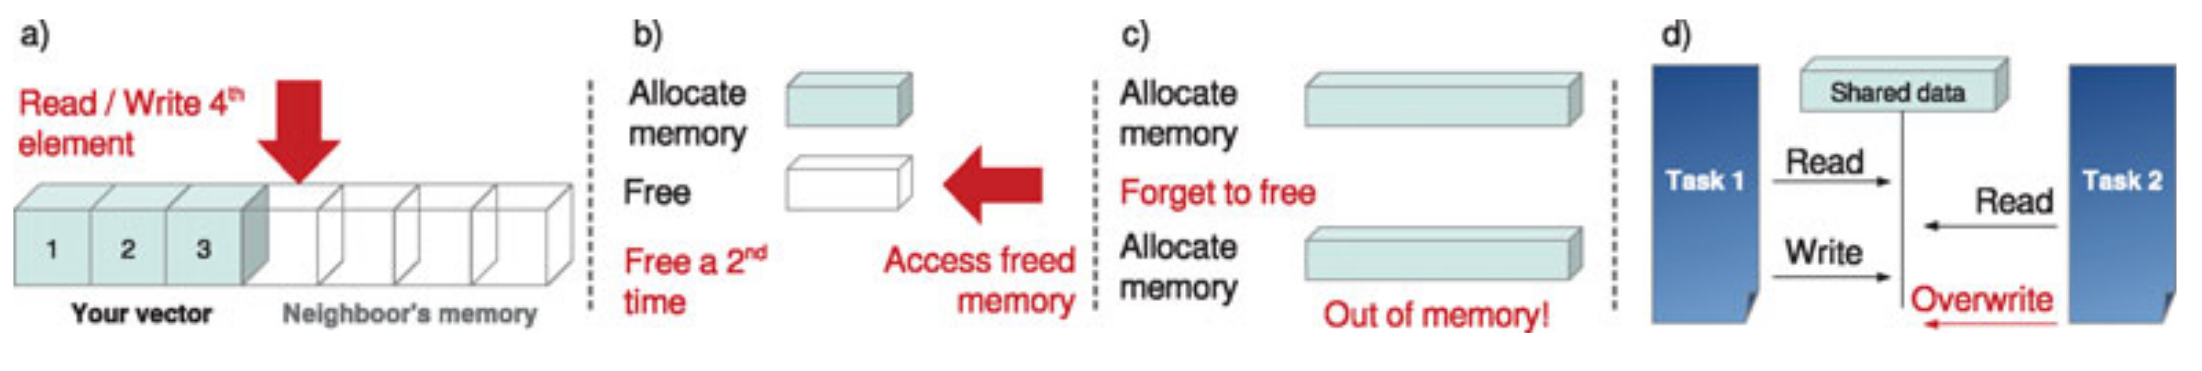
\includegraphics[width=\linewidth]{figures/memory-safety.png}
  \caption{`Potential Memory Safety Related Bugs'~\cite{blanco-cuaresma_bolmont_2016}. Reproduced with permission}
  \label{fig:mem}
\end{figure}

The programming language Rust, first released in 2014, attempts to solve the problem of memory safety, without compromising the programmer's ability to control memory usage. `[P]ure Rust programs are guaranteed to be free of memory errors (dangling pointers, doublefrees) as well as data races'~\cite{Matsakis:2014}. Rust is not the first programming language to offer some of these features~\cite{Manson:2005:JMM:1047659.1040336, pygc, jones1996concurrent}. However, it is one of the first languages to contain all of these memory features at the same time, whilst simultaneously delivering performance comparable to C and Fortran.

Some work has been done to investigate the applicability of Rust in scientific programming for bio-informatics~\cite{bioinformatics} and astro-physics~\cite{blanco-cuaresma_bolmont_2016}. Scientific kernels and apps such as the ones featured in these papers are common in HPC. The results of these investigations have been promising, and show that Rust is as fast, if not faster than implementations written in C or Fortran.

Rust's memory safety model does not allow the programmer to write unsafe code.

Rust's memory safety model also ensures that programmers do not need to use their time writing routines which are explicitly memory safe. Consider the listing below where we add four to a value after checking exists. In C we have to explicitly check if a value is null or not before proceeding with the operation. The programmer may forget to include this check, and potentially corrupt memory used by another part of the program.

\begin{lstlisting}[language=C]
// add_four.c

void add_four(int *foo){
  if(!foo){
    return;
  }
  *foo = *foo + 4;
}

void main{
  int *bar = 3;
  add_four(bar)
}
\end{lstlisting}
In comparison, the Rust version of this function needs no particular decoration to ensure that it is not carried out on an unexpected memory region. This is partly because Rust does not include null in the language. The closest equivalent that Rust has is the Option<T> type, like C++ std::optional<T>, which can either be \texttt{None} or \texttt{Some(value)}. This is very similar to Haskell's \texttt{Maybe} type. Rust forces the programmer to be mindful of when they might use a null type, and provides a simple, zero cost abstraction for dealing with it.
\begin{lstlisting}[language=Rust]
// add_four.rs
// MAKE FOO AN OPTION
fn add_four(foo: i32) -> i32{
  foo = foo + 4
}

fn main(){
  let bar = Some(3);
  bar.map(add_four);
}
\end{lstlisting}

Rust has many other features which are useful not just for general purpose programming, but HPC in particular. Rust's ownership memory model restricts values so that they can only ever by accessed through one owner, and must be explicitly borrowed to allow access. This leads to greater certainty about which process's functions are accessing which variables.
It is this memory model which allows parallel libraries like Rayon to exist. Rayon implements OpenMP style parallel loops, and because the rustc compiler is built on LLVM, it is able to efficiently vectorise code. Rust is certainly a strong contender for a HPC language, but it is as yet unproven. This dissertation project will aim to investigate how applicable Rust is to HPC. To acheive this aim, we will make use of mini-apps.

%Why mini apps
In high performance computing, `small self contained proxies for real applications' referred to as mini-apps~\cite{heroux2009improving}, are often used to test some particular configuration of a complex HPC stack~\cite{Mallinson:2014, Slaughter:2015}. As HPC systems and the applications which run on them are so complex, it is often difficult to accurately predict the performance of a HPC stack. This is a fundamental difficulty in comparing HPC configuration performances, and stastics comparing HPC clusters will often refer to a theoretical and a benchmarked performance~\cite{top500}.
%TODO expand this section

\chapter{Project Proposal} % What
Port a HPC mini app or benchmark into Rust. Document process and learning curve. Compare performance. Go into technical detail about how it works like it does.

draft mini app criteria, max around 1000 lines of C, not including driver code. what is rust like to program, i will reflect and inspect on writing in ownership model, compiler's feedback.

Mini app criteria, long list, how will i shortlist or choose from this
\section{Project Goals}
\begin{itemize}
  \item Find a software artifact that is representative of HPC use
  \item Port that software artefact to Rust
  \item Assess how easily C or C++ developers can understand Rust
  \item Find theoretical hardware capabilities
  \item Single Node Performance Tests
  \item Strech goal - Multi node performance test
  \item strech goal - 3 benchmarks
\end{itemize}
\chapter{Work plan} % How

Work item - thing that you get
Stretch goal - Rust MPI
\begin{description}
  \item[Introduction]:
  \begin{itemize}
    \item Current state of Programming Languages in HPC
    \item How are benchmarks/miniapps used in HPC
  \end{itemize}

  \item[Background]:
    \begin{itemize}
    \item What do programming languages need to be used in HPC?
    \item Why did D fail to replace C or C++ in HPC? What does this mean for Rust?
    \item What is Rust? What are its unique features of interest?
    \item How will my dissertation provide an indication of Rust's ability to succeed in HPC?
  \end{itemize}
  \item[Methods]
  \item[Implementation]:
  \begin{itemize}
    \item Overview of Software which I will port
    \item Technical description of my implementation
    \item Discussion of what implementation and learning Rust was like
    \item Correctness testing
  \end{itemize}
  \item[Performance Analysis]:
  \begin{itemize}
    \item How does performance compare to original app?
    \item How close do we get to hardware limit?
    \item Why does performance differ? (potentially go onto machine code analysis)
    \item How are both implementations affected by scaling?
  \end{itemize}
  \item[Programmable]:
  \begin{itemize}
    \item Did I like programming in Rust?
    \item Can other people understand it?
  \end{itemize}
  \item[Conclusion] :
  \begin{itemize}
    \item Summary of findings
    \item Further work
  \end{itemize}
\end{description}

Gantt Chart to go here

\chapter{Risk Analysis}
In planning our project, we have endevoured to be aware of all risks to the project which are potential and plausible. We collected these risks through consultation with our dissertation supervisor and fellow students. We present these risks in our risk register (table~\ref{tab:risk}).

The most likely risk in the risk register is risk 3. It is normal for dissertation students to be given technical support in their dissertation projects by their dissertation supervisors and EPCC with relavent domain knowledge. However, in our case the available technical support is likely to be more limited, as Rust is not a well known programming language amongst EPCC staff. Our mitigation for this risk is to rely upon the Rust community for issues which are particular to the Rust language. We do not expect the Rust community have a great deal of knowledge in the HPC space, but our expectation is that EPCC staff will be able to provide the necessary HPC expertise for us, whilst the Rust community provides guidance on the Rust language. It will fall to us to synthesise this knowledge where necessary, which is well within the objectives of this dissrtation.

\section{Risk Register}
We intend to update the risk register at weekly intervals throughout the project lifetime, in an effort to remain cogniscant of risks and make necessary adjustments to our work plan.

\begin{table}[h]
  \centering
  \begin{tabular}{c | p{4cm} c c p{4cm}}
  ID & Risk & Probability & Severity & Mitigation \\
    \hline
  1 &  Poor port selection & Medium & Medium & Confirm selection with advisers \\ \hline
  2 &  No knowledge of Rust amongst EPCC staff & High & Low & Rely on Rust community for language issues \\
    \hline
  3&  Rust Community has poor knowledge of HPC considerations & Medium & Low & No mitigation. We will have to take this risk and work around it. \\
    \hline
4 &    Run out of time for multiple node performance tests & Medium & Low & Jettison this goal. \\
\hline
5 & Run out of time to implement all benchmarks & Medium & Low & Drop benchmark. \\
    \end{tabular}
  \caption{Risk Register}
  \label{tab:risk}
\end{table}
\chapter{Preliminary Findings}
Thus far the work done in this project has been exploratory. We have implemented a simple program in C and in Rust, and compared performance. The program was a simple SAXPY (Single precision A-X plus Y) performed on a large array of random digits. We were not able to use this program to accurately compare the two programs, as we found Rust's aggressive \texttt{--release} optimisation (similar in intent to \texttt{-O3} found in C compilers) removed much of the processing done by the loop. This exercise illustrated to us some of the difficulties inherit in comparing two programming languages. Not only did we find proof that compiled programs are not wholly representative of their source code, we also found that `translating' a program from one language to another had its own pitfalls and considerations. We had to consider whether to use follow Rust idioms, like using iterators, or instead remaining more faithful to the C implementation and using a loop to increment a variable to access an array value. Ultimately, we have decided to write idiomatic, or Rustic Rust, unless there is more performant way to express the code.

We have made this decision because, as both C and Rust are turing complete, Rust can express the same algorithms as C, especially through the use of unsafe Rust. Unsafe Rust is a subset of the Rust programming language which allows users to avoid Rust's strict memory model. If we write Rust to be like C, and especially if we write it in a way to avoid or minimise the features of Rust, then the comparison between implementations becomes dishonest. However, we feel it is fair to deviate from idiomatic Rust where there are noticable performance benefits and that deviation is minimal, due to the great emphasis HPC programmers place on performance.

We have installed Rust on Cirrus and compiled and run the simple SAXPY program mentioned above. We have also found the Rust package management system, cargo, to work with no required set up. This package system is similar to python's pip or Node JS's npm and does not require administrator privaleges. We believe this will be useful to HPC developers, as many Rust follows a `batteries not included' philosophy, requiring users to download and install packages for common utilities like random number generation. Alongside our simple programs, we have compiled some complex Rust programs with higher number of dependencies~\cite{Bat,Exa}.

\begin{itemize}
  \item formal criteria for what makes a HPC language
  \item research has found rust to fit some criteria for becoming a HPC language
  \item Rust has been installed on Cirrus
  \item Rust ownership and borrowing has been explored. (should I include saxpy fragment)
  \item Rust is capable of very aggressive optimisation
  \item List some Interesting potential HPC features in rust
\end{itemize}


\chapter{Conclusion}
Should i refer to the whole document, or ignore the diss review?

In conclusion, I think this diss will be fun. Reviewing the dissertations has made me consider my performance process, and how I will structure my own dissertation.
\pagebreak
\bibliographystyle{plain}
\bibliography{bib}
\end{document}
